\section{混合智能问答系统}
\zihao{-4}
\label{section:mixed-system}

\subsection{意图识别}
\label{subsection:task-recognition}

如节\ref{section:peer-system}中所述,在线呼叫中心的客服领域普遍采用的是检索式智能问答系统。
该系统首先对顾客问题进行语法、语义分析,抽取关键词的组合,通过进行关键词组合的扩展确定问题类别和顾客问题意图;
然后连接本地/网络知识库对顾客意图进行检索,抛出补全信息请求应答或确定候选结果集;
接着对候选结果集进行排序,获取分值或概率最高的结果,将结果信息进行整合,抛出最终应答。

对于检索式智能问答系统,正确识别顾客问题意图是后续检索和反馈正确应答的关键。
目前的意图识别主要依赖问答系统用户即商家连接或自建的问题词库,根据该词库抽取关键词进而汇集关键词的组合完成意图识别。
在此过程中,往往会出现由于用户输入错字导致关键词抽取失败,或是长问句内包含多个问题以致无法准确
完成意图识别。

对于用户输入错字的问题,
由于基于词库或词典抽取关键词的特性,如果词库中没有包含错别字的组合,如表\ref{table:jimi-skill}中所举“优汇劵”和“优惠卷”,
词库包含“优惠卷”而不包含“优汇劵”,顾客若输入“优汇劵”则导致关键词“优惠卷”失败,无法完成意图识别。

值得注意的是,在输入错字的情况下,由于汉语拼写和输入的特性,一些规律是可以被归纳和利用的。
顾客输入的错误关键词和正确关键词往往是拼音相同或相近的,这种相同和相近在一定程度上反映了错误关键词和正确关键词的距离。
而传统的文本分聚类往往忽视了拼音上的距离,
仅考虑词在整个文档或训练集中出现的频率并将这种统计信息转化为词向量权值,如TF-IDF方法,
训练集样本本身对此方法有较大影响,易出现拟合,降低模型的泛化能力。
单纯考虑错误关键词与正确关键词的拼音相似度也是不可取的,对于多字组合的关键词,其拼音完全相似的词集数为字各自拼音完全相似的词集数之积,
因此综合考虑词的统计信息与拼音相似度作为其向量权值是一种预期效果较优的向量化方法。

在明确了词向量化方法后,此时关键词的识别可转化为对应不同关键词的多分(聚)类问题,完成知识库(词库)的扩充,实现关键词的识别。
通过结合关键词的句法依存结构分析\citep{问题识别},完成长文句内多问题的切分,进而实现用户输入错字下和长问句下的意图识别。

\subsection{端到端学习}

基于检索式问答系统一般针对用户的自然语言问句,提供准确的应答。
例如,对于问句“泰戈尔的出生地在哪儿?”,返回“加尔各答”。
但是,仅仅提供这种孤零零的答案实体并不是非常友好的交互方式,用户更希望接受类人的回答,
如以自然语言表示的完整答案(以下简称自然应答),“印度诗人泰戈尔出生于加尔各答市”。

单纯生成自然应答的生成式问答系统往往被应用在无任务驱动的聊天场景。
在这种场景下,用户没有明确的目标,不需要获取某种准确的信息,因此很少涉及到对知识库的检索。
如何检索知识库中的已有知识生成能够准确问答问题且流利的自然应答是一种挑战。

\begin{figure*}[!htp]
    \centering
    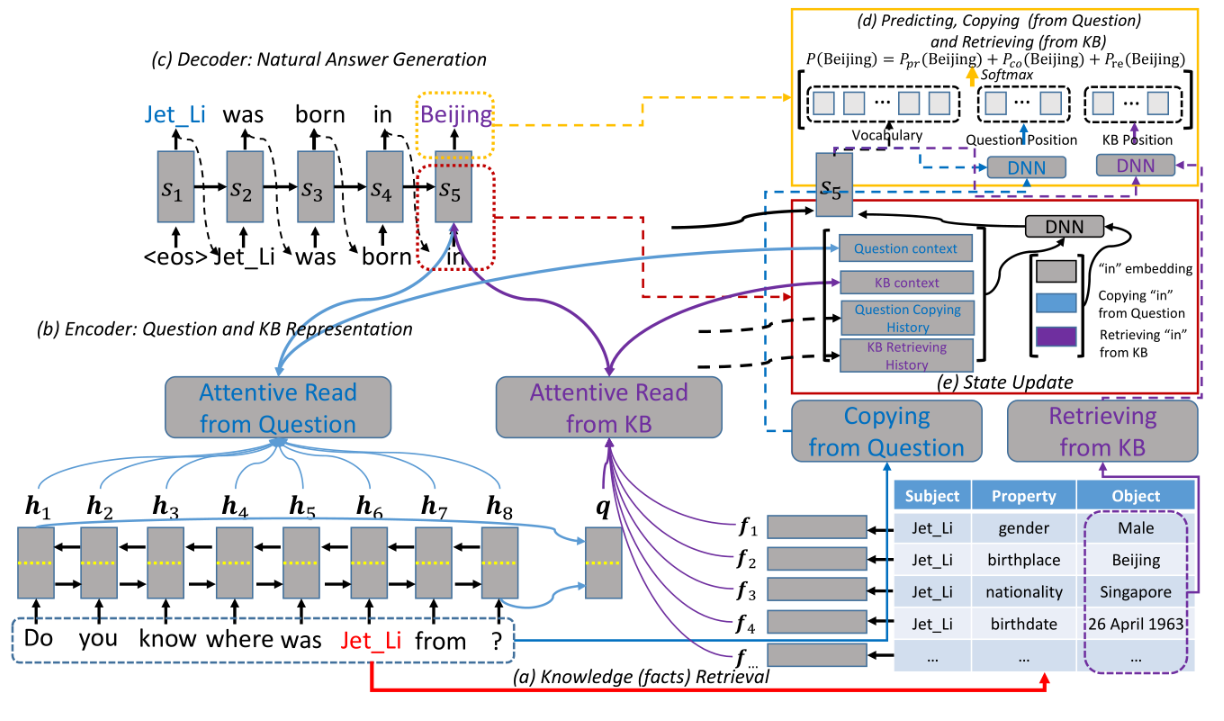
\includegraphics[width=0.8\textwidth]{mixed_system.png}
    \caption{\label{figure:mixed_system} 自然答案生成系统}
\end{figure*}
为解决此问题,中科院自动化所的何世柱博士等\citep{hegenerating}提出了一个端到端的问答系统。
如图\ref{figure:mixed_system}中“Do you know where was Jet Li from?”为例进行阐述。

首先对问句进行语义分析,抽取出关键词,连接知识库进行检索,获取到与李连杰相关的知识实体;
然后基于双向循环神经网络Bi-RNN的Encoder-Decoder机制对问句进行问题编码,
对知识库检索结果进行知识编码;
接着根据问题和知识的编码向量来生成自然答案。
自然答案虽然是词序列,但是不同的词可能需要通过不同途径获得。
例如,对于上述问题的答案“Jet Li was born in Beijing”,
词语“Jet Li ”需要从源问句中拷贝得到,实体词“Beijing”需要从知识库中检索得到,
而其他词如“born”、“in”等需要通过模型预测得到。
因此,这里在标准的序列到序列(Sequence-to-Sequence)模型基础上,
融合了三种词语获得模式(包括拷贝、检索和预测),
用统一的模型对其建模,
让各种模式之间相互竞争相互影响,
最终对问题生成一个最优的自然答案。

值得注意的是,该模型一方面仅以当前语句进行Encoder没有考虑上下文,无法进行上下文关联。
另一方面,由于关键词是问句中抽取,相关直接从知识库中直接拷贝,若输入错别字,则同样会造成生成失败的情况。
因此改模型可从两方面进行改进,一是结合小节\ref{subsection:task-recognition}中的意图识别方法,对关键词词库进行扩充,
实现关键词的正确抽取;二是考虑多轮对话情景,引入Gated RNN Unit对进行上文记忆和下文推演,以生成更好的自然语言应答。